\section*{Introduction}

FracNoise is a C library providing structures and functions to generate noise based on the Perlin noise.\\ 

The library provides the structure PerlinNoise and its functions to generate noise as described by Prof. Ken Perlin.\\

It also provides the structure FracNoise and its functions, which extends the PerlinNoise. A FracNoise is made of a composition of one or several PerlinNoise. Each of the composed PerlinNoise can be individually controled over its input/output values scale and shift; be attached to a boundary (Shapoid) outside of which the PerlinNoise is inactive, and inside of which it becomes smoothly active across a border width defined by the user; support a recursive definition with user defined depth and strength; have a 'smooth' parameter to set the aspect (round or spiky) of the PerlinNoise; have a user defined seed; return output as a vector of any dimension; take input as a vector of 1, 2 or 3 dimensions, however the limit of 3 can somehow be extended up to 6 by using the 3 components of the seed as input values too.\\

The FracNoise structure also provides an export function toward ".df3" density file to be used in computer graphics software like POV-Ray.\\ 

It uses the \begin{ttfamily}PBErr\end{ttfamily}, the \begin{ttfamily}GSet\end{ttfamily}, the \begin{ttfamily}Shapoid\end{ttfamily} and the \begin{ttfamily}PBMath\end{ttfamily} library.\\

\section{Definitions}

\subsection{Perlin noise}

For details about the Perlin noise, please refer to the paper of, and its reference implementation by, Prof. Ken Perlin:\\
http://mrl.nyu.edu/\textasciitilde perlin/paper445.pdf\\
http://mrl.nyu.edu/\textasciitilde perlin/noise/\\

The implementation of the Perlin noise in the FracNoise library is a port from the JAVA Reference Implementation of Prof. Perlin toward C language with only modification a mapping of the output value to [0.0, 1.0].\\

\subsection{FracNoise}

In the FracNoise structure, each instance of a PerlinNoise is called a PerlinNoisePod. A PerlinNoisePod contains a PerlinNoise and the associated parameters. These parameters are described below:\\
\begin{itemize}
\item seed: a 3D vector of float values.\\
The value returned by the PerlinNoise is defined by the permutations used to init the structure. Then a given input will always generates the same output, which is not very useful. Different output values would require to generate different permutations. FracNoise offers another solution: Each PerlinNoise is associated to a seed which is used to transform the input values. The transformation is a rotation of the input vector around the axis defined by the seed vector. The seed vector is a 3D vector, and the input is extended internally to a 3D vector if necessary (missing components equal 0.0). The angle of the rotation for the $i$-th component of the output value is defined as $2\pi(i+1)/(n+1)$ where $n$ is the dimension of output. Then, we can generate as many different noises as needed, and we solve at the same time the problem of generating output of dimension higher than 1. Also, the seed components can be used as extra components to the input when one needs more than 3D input. As the transformation is a 3D rotation of the input, continuity and derivability of the output are conserved over seed values.
\item scaleIn: a vector of float values of dimension equals to the dimension of the input.\\
This scale is applied to the input, component by component.
\item fractalLvl: an integer greater than or equal to 0.\\
The fractal level controls the number of recursive call of the PerlinNoise on itself. If it's equal to 0, the output is the standard output. If it's equal to 1 the output is equal to the standard output added to the output of the same PerlinNoise multiplied by the fractal coefficient (see below) for input divided by the fractal coefficient. And so on (there is no limit to the fractal level). Recursive call are made before applying the scaling and shifting on output. As the output at each level sum up, the final output value might get out of the range [0.0, 1.0], but it is automatically rescaled to ensure the values stay in the correct range whatever the fractal level. Recursive call occurs before smoothing, scaling and shifting.
\item fractalCoeff: a float value (typically in ]0.0, 1.0[ but one may experiments with values out of this range).\\
The output value is multiplied by the fractal coefficient at each fractal level, and the input value is divided by the fractal coefficient at each level. the output value is rescaled to ensure it stays inside [0.0,1.0]. So for example, for a PerlinNoise with a fractal level of 2, a fractal coefficient of 0.1, an input value of 0.5, the output value will be equal to (PerlinNoise(0.5)*0.9+0.1*PerlinNoise(5.0))*0.9+0.01*PerlinNoise(50.0)
\item smooth: a float value greater than 0.0.\\
The smooth is applied after fractal and before scaling.Output values are raise to the power of smooth component by component. This can be used to control the general aspect of the distribution of the output values (more bumpy for value below 1.0, more thorny for value above).
\item square: a float value greater in [0.0, 1.0].\\
The squareness of the pod controls the smoothing of the input value of the PerlinNoise. If it equals 0.0 the result is the standard PerlinNoise. If it equals 1.0 the result is the PerlinNoise without smoothing of the input. Explicitly: $smooth(t,square)=(1-square)smooth(t)+square*t$. The squareness is applied when calculating the PerlinNoise for a pod with this pod's squareness.\\
\item bound: a Shapoid.\\
The PerlinNoise is defined over $\mathbb{R}$, however one can want to restrain it to some subdomain. This can be done by attaching a Shapoid with proper position and axis of dimension equal to the input dimension. Then, the PerlinNoise will output 0.0 for input (original one, not the scaleIn-ed one) outside of the subdomain defined by the outside of the Shapoid, and its normal value for the subdomain defined by the inside of the Shapoid.
\item border: a float value between 0.0 and 1.0 representing the border of the boundary.\\
If the PerlinNoise is attached to a boundary, one may want a smooth transition between the outside and inside of the boundary. The depth in the Shapoid defining the boundary of the input position is compared to the border, if the depth is greater than the border then the normal output is returned. If the depth is between 0.0 and the border, the normal output is multiplied by SmootherStep(depth/border).
\item scaleOut: a vector of float values of dimension equals to the dimension of the output.\\
This scale is applied to the output, component by component.
\item shiftOut: a vector of float values of dimension equals to the dimension of the output.\\
This shift is added to the output after scaling.
\end{itemize}

The value of a FracNoise for a given input is equal to the sum of the values of its PerlinNoisePod for this input and can be expressed as follow:\\

\begin{equation}
\begin{array}{l}
FracNoise(\overrightarrow{p})=\\
\sum_{pod}\left(
  \left(
    In(\overrightarrow{p}).
    \left(
      \sum_{f=0}^lc^f
      \left[
        PN\left(
          Rot_{\overrightarrow{e}}\left(
            \overrightarrow{p}\odot\overrightarrow{si},\frac{2\pi(i+1)}{n+1}          
          \right).\frac{1.0}{c^f},q
        \right)^s
      \right]_{i\in[0,n-1]}
      \odot \overrightarrow{so}+\overrightarrow{t}
    \right)
  \right)
\right)
\end{array}
\end{equation}

where\\
\begin{itemize}
\item $\overrightarrow{p}$ is the input (redimensioned to a 3D vector if it's of different dimension).
\item $pod$ is the set of PerlinNoisePod.
\item $In(\overrightarrow{p})$ is the insideness of $\overrightarrow{p}$, equals to 1.0 if the PerlinNoisePod has no boundary, or if it has a boundary: 0.0 if $\overrightarrow{p}$ is out of boundary; 1.0 if $depth(\overrightarrow{p})$ is greater than the $border$ of the PerlinNoisePod; SmootherStep($depth(\overrightarrow{p})/border$) else. We remind that\\ SmootherStep(x)=$((6x-15)x+10)x^3$.
\item $l$ is the fractalLvl.
\item $c$ is the fractalCoeff.
\item $PN()$ is the PerlinNoise function.
\item $\overrightarrow{e}$ is the seed.
\item $Rot_{\overrightarrow{e}}(\overrightarrow{p}, \theta)$ is the rotation of $\overrightarrow{p}$ around the axis $\overrightarrow{e}$ by angle $\theta$.
\item $\overrightarrow{si}$ is the scaleIn.
\item $\overrightarrow{so}$ is the scaleOut.
\item $\overrightarrow{t}$ is the shiftOut.
\item $n$ is the number of dimensions of output.
\item $s$ is the smoothness of the pod.
\item $q$ is the squareness of the pod.
\end{itemize}

\section{Interface}

\begin{scriptsize}
\begin{ttfamily}
\verbatiminput{/home/bayashi/GitHub/FracNoise/fracnoise.h}
\end{ttfamily}
\end{scriptsize}

\section{Code}

\subsection{fracnoise.c}

\begin{scriptsize}
\begin{ttfamily}
\verbatiminput{/home/bayashi/GitHub/FracNoise/fracnoise.c}
\end{ttfamily}
\end{scriptsize}

\subsection{fracnoise-inline.c}

\begin{scriptsize}
\begin{ttfamily}
\verbatiminput{/home/bayashi/GitHub/FracNoise/fracnoise-inline.c}
\end{ttfamily}
\end{scriptsize}

\section{Makefile}

\begin{scriptsize}
\begin{ttfamily}
\verbatiminput{/home/bayashi/GitHub/FracNoise/Makefile}
\end{ttfamily}
\end{scriptsize}

\section{Unit tests}

\begin{scriptsize}
\begin{ttfamily}
\verbatiminput{/home/bayashi/GitHub/FracNoise/main.c}
\end{ttfamily}
\end{scriptsize}

\section{Unit tests output}

\begin{scriptsize}
\begin{ttfamily}
\verbatiminput{/home/bayashi/GitHub/FracNoise/unitTestRef.txt}
\end{ttfamily}
\end{scriptsize}

UnitTestPerlinNoise2DRef.png:\\
\begin{center}
\begin{figure}[H]
\centering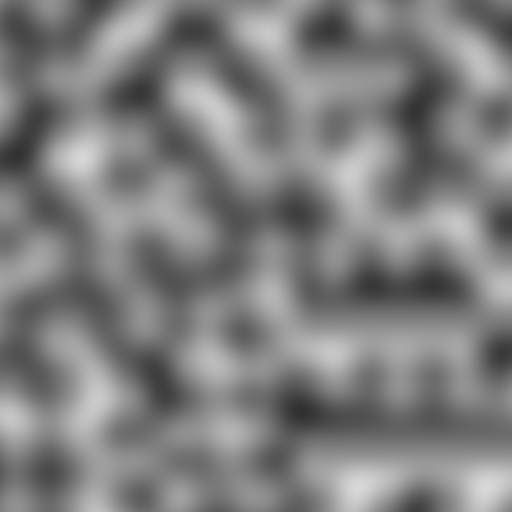
\includegraphics[width=6cm]{./UnitTestPerlinNoise2DRef.png}\\
\end{figure}
\end{center}

UnitTestPerlinNoise3DRef.png:\\
\begin{center}
\begin{figure}[H]
\centering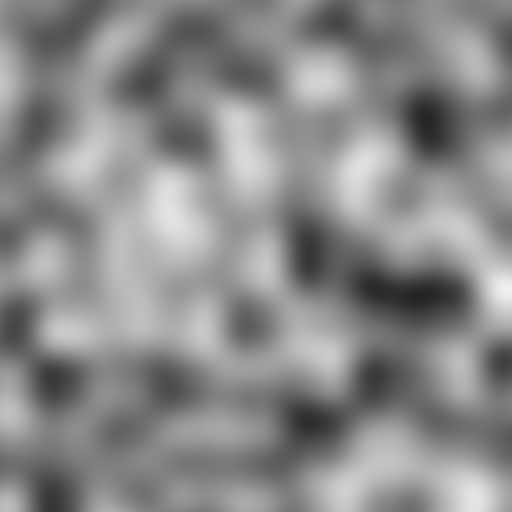
\includegraphics[width=6cm]{./UnitTestPerlinNoise3DRef.png}\\
\end{figure}
\end{center}

UnitTestFracNoiseGetRef.png:\\
\begin{center}
\begin{figure}[H]
\centering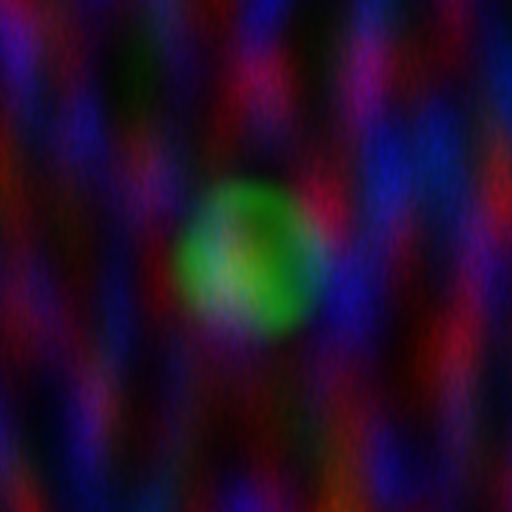
\includegraphics[width=6cm]{./UnitTestFracNoiseGetRef.png}\\
\end{figure}
\end{center}

UnitTestFracNoiseExportRef.df3 (rendered in POV-Ray in a unit cube):\\
\begin{center}
\begin{figure}[H]
\centering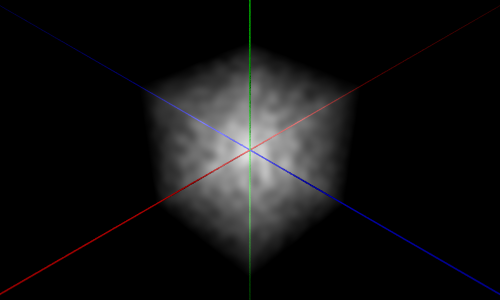
\includegraphics[width=6cm]{./DF3.png}\\
\end{figure}
\end{center}

\section{Examples}

\subsection{Terrain}

main.c:\\
\begin{scriptsize}
\begin{ttfamily}
\verbatiminput{/home/bayashi/GitHub/FracNoise/Examples/Terrain/main.c}
\end{ttfamily}
\end{scriptsize}

terrain.pov:\\
\begin{scriptsize}
\begin{ttfamily}
\verbatiminput{/home/bayashi/GitHub/FracNoise/Examples/Terrain/terrain.pov}
\end{ttfamily}
\end{scriptsize}

HF.png:\\
\begin{center}
\begin{figure}[H]
\centering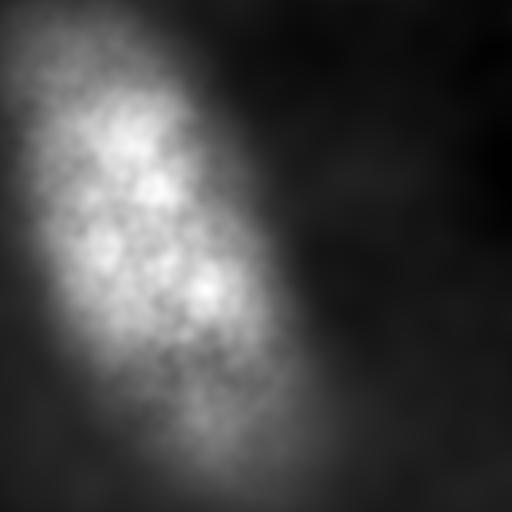
\includegraphics[width=6cm]{./HF.png}\\
\end{figure}
\end{center}

terrain.png:\\
\begin{center}
\begin{figure}[H]
\centering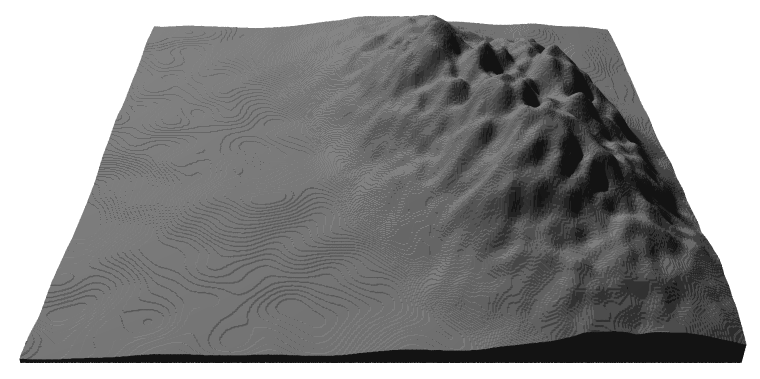
\includegraphics[width=6cm]{./terrain.png}\\
\end{figure}
\end{center}

\subsection{Cloud}

main.c:\\
\begin{scriptsize}
\begin{ttfamily}
\verbatiminput{/home/bayashi/GitHub/FracNoise/Examples/Cloud/main.c}
\end{ttfamily}
\end{scriptsize}

cloud.pov:\\
\begin{scriptsize}
\begin{ttfamily}
\verbatiminput{/home/bayashi/GitHub/FracNoise/Examples/Cloud/cloud.pov}
\end{ttfamily}
\end{scriptsize}

cumulusA.png:\\
\begin{center}
\begin{figure}[H]
\centering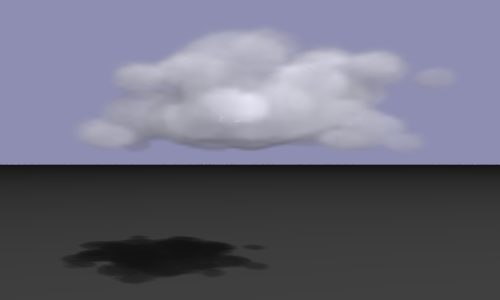
\includegraphics[width=6cm]{./cumulusA.png}\\
\end{figure}
\end{center}

cumulusB.png:\\
\begin{center}
\begin{figure}[H]
\centering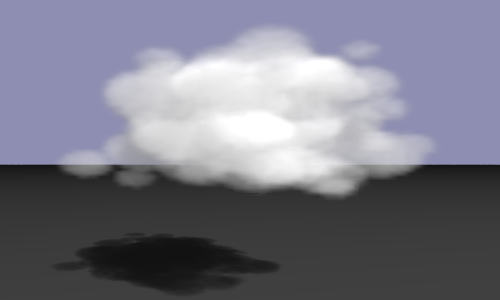
\includegraphics[width=6cm]{./cumulusB.png}\\
\end{figure}
\end{center}

stratusA.png:\\
\begin{center}
\begin{figure}[H]
\centering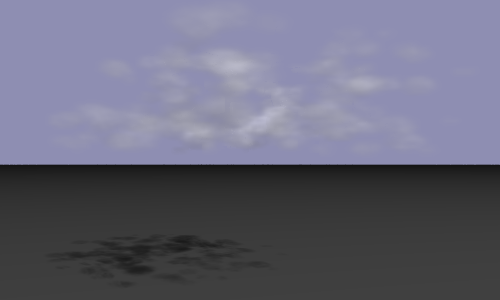
\includegraphics[width=6cm]{./stratusA.png}\\
\end{figure}
\end{center}

stratusB.png:\\
\begin{center}
\begin{figure}[H]
\centering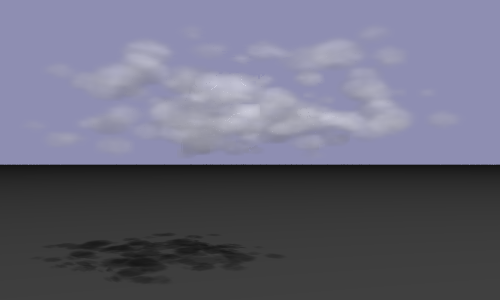
\includegraphics[width=6cm]{./stratusB.png}\\
\end{figure}
\end{center}

stratusC.png:\\
\begin{center}
\begin{figure}[H]
\centering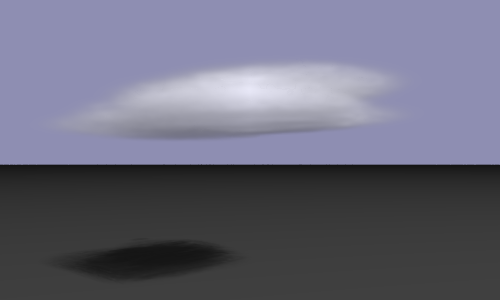
\includegraphics[width=6cm]{./stratusC.png}\\
\end{figure}
\end{center}

\subsection{Rock}

main.c:\\
\begin{scriptsize}
\begin{ttfamily}
\verbatiminput{/home/bayashi/GitHub/FracNoise/Examples/Rock/main.c}
\end{ttfamily}
\end{scriptsize}

rock.pov:\\
\begin{scriptsize}
\begin{ttfamily}
\verbatiminput{/home/bayashi/GitHub/FracNoise/Examples/Rock/rock.pov}
\end{ttfamily}
\end{scriptsize}

rock01.png:\\
\begin{center}
\begin{figure}[H]
\centering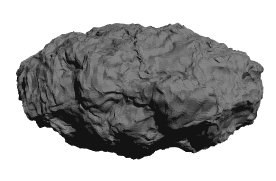
\includegraphics[width=6cm]{./rock01.png}\\
\end{figure}
\end{center}

rock03.png:\\
\begin{center}
\begin{figure}[H]
\centering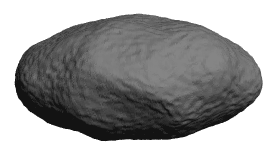
\includegraphics[width=6cm]{./rock03.png}\\
\end{figure}
\end{center}

rock05.png:\\
\begin{center}
\begin{figure}[H]
\centering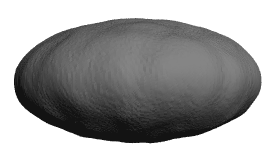
\includegraphics[width=6cm]{./rock05.png}\\
\end{figure}
\end{center}

rock06.png:\\
\begin{center}
\begin{figure}[H]
\centering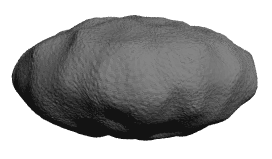
\includegraphics[width=6cm]{./rock06.png}\\
\end{figure}
\end{center}

rock30.png:\\
\begin{center}
\begin{figure}[H]
\centering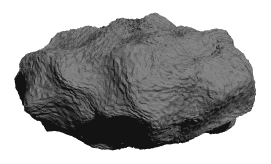
\includegraphics[width=6cm]{./rock30.png}\\
\end{figure}
\end{center}

rock50.png:\\
\begin{center}
\begin{figure}[H]
\centering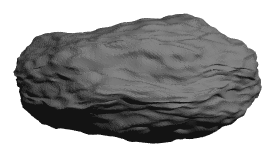
\includegraphics[width=6cm]{./rock50.png}\\
\end{figure}
\end{center}

